\tikzset{every picture/.style={line width=0.75pt}} %set default line width to 0.75pt        

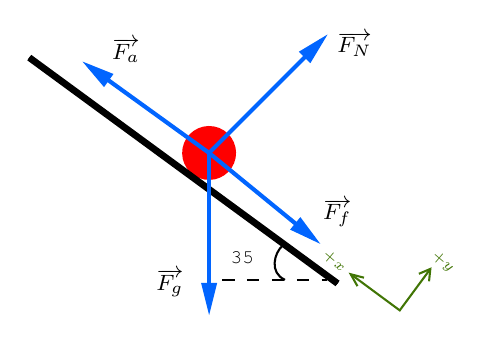
\begin{tikzpicture}[x=0.75pt,y=0.75pt,yscale=-1,xscale=1]
	%uncomment if require: \path (0,300); %set diagram left start at 0, and has height of 300

	%Shape: Ellipse [id:dp1428949648769431] 
	\draw  [color={rgb, 255:red, 255; green, 0; blue, 0 }  ,draw opacity=1 ][fill={rgb, 255:red, 254; green, 0; blue, 0 }  ,fill opacity=1 ] (198.05,181.45) .. controls (199.28,174.66) and (194.78,168.16) .. (188,166.92) .. controls (181.21,165.69) and (174.71,170.19) .. (173.47,176.97) .. controls (172.24,183.76) and (176.74,190.26) .. (183.52,191.5) .. controls (190.31,192.73) and (196.81,188.23) .. (198.05,181.45) -- cycle ;
	%Shape: Rectangle [id:dp48287918810377195] 
	\draw   (247.91,240.87) -- (100.19,132.64) -- (99.74,133.25) -- (247.46,241.49) -- cycle ;
	%Shape: Rectangle [id:dp005233673921997584] 
	\draw   (247.46,241.49) -- (99.74,133.25) -- (99.29,133.87) -- (247.01,242.1) -- cycle ;
	%Shape: Rectangle [id:dp9526931686132831] 
	\draw   (247.01,242.1) -- (99.29,133.87) -- (98.85,134.48) -- (246.56,242.71) -- cycle ;

	%Straight Lines [id:da8350690671631047] 
	\draw [color={rgb, 255:red, 1; green, 101; blue, 255 }  ,draw opacity=1 ][line width=1.5]    (185.76,179.21) -- (185.76,253.35) ;
	\draw [shift={(185.76,257.35)}, rotate = 270] [fill={rgb, 255:red, 1; green, 101; blue, 255 }  ,fill opacity=1 ][line width=0.08]  [draw opacity=0] (15.6,-3.9) -- (0,0) -- (15.6,3.9) -- cycle    ;
	%Straight Lines [id:da1062981577052522] 
	\draw [color={rgb, 255:red, 1; green, 101; blue, 255 }  ,draw opacity=1 ][line width=1.5]    (185.76,179.21) -- (239.99,124.98) ;
	\draw [shift={(242.82,122.15)}, rotate = 135] [fill={rgb, 255:red, 1; green, 101; blue, 255 }  ,fill opacity=1 ][line width=0.08]  [draw opacity=0] (15.6,-3.9) -- (0,0) -- (15.6,3.9) -- cycle    ;
	%Straight Lines [id:da21972886949175963] 
	\draw [color={rgb, 255:red, 1; green, 101; blue, 255 }  ,draw opacity=1 ][line width=1.5]    (185.76,179.21) -- (128.01,137.53) ;
	\draw [shift={(124.77,135.19)}, rotate = 35.82] [fill={rgb, 255:red, 1; green, 101; blue, 255 }  ,fill opacity=1 ][line width=0.08]  [draw opacity=0] (15.6,-3.9) -- (0,0) -- (15.6,3.9) -- cycle    ;
	%Shape: Right Angle [id:dp7929492774408056] 
	% \draw  [color={rgb, 255:red, 65; green, 117; blue, 5 }  ,draw opacity=1 ][line width=0.75]  (281.02,261.19) -- (255.11,241.93) -- (271.45,219.97) ;
	% \draw  [color={rgb, 255:red, 65; green, 117; blue, 5 }  ,draw opacity=1 ] (265.4,222.48) -- (271.49,219.9) -- (270.8,226.48) ;
	% \draw  [color={rgb, 255:red, 65; green, 117; blue, 5 }  ,draw opacity=1 ] (277.33,255.08) -- (281.14,261.33) -- (274.03,259.73) ;
	\draw  [color={rgb, 255:red, 65; green, 117; blue, 5 }  ,draw opacity=1 ][line width=0.75]  (254.14,237.71) -- (277.61,255.05) -- (292.31,235.15) ;
	\draw  [color={rgb, 255:red, 65; green, 117; blue, 5 }  ,draw opacity=1 ] (291.72,241.04) -- (292.35,235.09) -- (286.84,237.43) ;
	\draw  [color={rgb, 255:red, 65; green, 117; blue, 5 }  ,draw opacity=1 ] (260.39,239.3) -- (253.99,237.65) -- (257.24,243.38) ;


	%Straight Lines [id:da0016552996956802346] 
	\draw [color={rgb, 255:red, 1; green, 101; blue, 255 }  ,draw opacity=1 ][line width=1.5]    (185.76,179.21) -- (236.24,220.47) ;
	\draw [shift={(239.33,223)}, rotate = 219.26] [fill={rgb, 255:red, 1; green, 101; blue, 255 }  ,fill opacity=1 ][line width=0.08]  [draw opacity=0] (15.6,-3.9) -- (0,0) -- (15.6,3.9) -- cycle    ;
	%Curve Lines [id:da5437896212575373] 
	\draw    (221.33,223.67) .. controls (217,227.33) and (214.67,237) .. (222.33,240.33) ;
	%Straight Lines [id:da6898758265813036] 
	\draw  [dash pattern={on 4.5pt off 4.5pt}]  (192,240.33) -- (242.33,240.33) ;

	% Text Node
	\draw (158.85,233.91) node [anchor=north west][inner sep=0.75pt]  [font=\footnotesize] [align=left] {$\displaystyle \overrightarrow{F_{g}}$};
	% Text Node
	\draw (137.56,122.62) node [anchor=north west][inner sep=0.75pt]  [font=\footnotesize] [align=left] {$\displaystyle \overrightarrow{F_{a}}$};
	% Text Node
	\draw (246.09,119.35) node [anchor=north west][inner sep=0.75pt]  [font=\footnotesize,color={rgb, 255:red, 0; green, 0; blue, 0 }  ,opacity=1 ] [align=left] {$\displaystyle \overrightarrow{F_{N}}$};
	% Text Node
	\draw (239.23,199.96) node [anchor=north west][inner sep=0.75pt]  [font=\footnotesize] [align=left] {$\displaystyle \overrightarrow{F_{f}}$};
	% Text Node
	\draw (194.67,225) node [anchor=north west][inner sep=0.75pt]  [font=\scriptsize] [align=left] {{\fontfamily{pcr}\selectfont 35}$\displaystyle \degree $};
	% % Text Node
	% \draw (285.99,258.65) node [anchor=north west][inner sep=0.75pt]  [font=\tiny,color={rgb, 255:red, 65; green, 117; blue, 5 }  ,opacity=1 ,rotate=-40.39] [align=left] {$\displaystyle +x$};
	% % Text Node
	% \draw (274.67,208.71) node [anchor=north west][inner sep=0.75pt]  [font=\tiny,color={rgb, 255:red, 65; green, 117; blue, 5 }  ,opacity=1 ,rotate=-40.39] [align=left] {$\displaystyle +y$};

	% Text Node
	\draw (242.99,223.32) node [anchor=north west][inner sep=0.75pt]  [font=\tiny,color={rgb, 255:red, 65; green, 117; blue, 5 }  ,opacity=1 ,rotate=-40.39] [align=left] {$\displaystyle +x$};
	% Text Node
	\draw (295.67,223.71) node [anchor=north west][inner sep=0.75pt]  [font=\tiny,color={rgb, 255:red, 65; green, 117; blue, 5 }  ,opacity=1 ,rotate=-40.39] [align=left] {$\displaystyle +y$};

\end{tikzpicture}